\documentclass[11pt,compress,t,notes=noshow, aspectratio=169, xcolor=table]{beamer}

\usepackage[nospeakermargin]{../../style/lmu-lecture-2}
% Defines macros and environments
% This file is included in slides and exercises

% Rarely used fontstyle for R packages, used only in 
% - forests/slides-forests-benchmark.tex
% - exercises/single-exercises/methods_l_1.Rnw
% - slides/cart/attic/slides_extra_trees.Rnw
\newcommand{\pkg}[1]{{\fontseries{b}\selectfont #1}}

% Spacing helpers, used often (mostly in exercises for \dlz)
\newcommand{\lz}{\vspace{0.5cm}} % vertical space (used often in slides)
\newcommand{\dlz}{\vspace{1cm}}  % double vertical space (used often in exercises, never in slides)
\newcommand{\oneliner}[1] % Oneliner for important statements, used e.g. in iml, algods
{\begin{block}{}\begin{center}\begin{Large}#1\end{Large}\end{center}\end{block}}

% Don't know if this is used or needed, remove?
% textcolor that works in mathmode
% https://tex.stackexchange.com/a/261480
% Used e.g. in forests/slides-forests-bagging.tex
% [...] \textcolor{blue}{\tfrac{1}{M}\sum^M_{m} [...]
% \makeatletter
% \renewcommand*{\@textcolor}[3]{%
%   \protect\leavevmode
%   \begingroup
%     \color#1{#2}#3%
%   \endgroup
% }
% \makeatother


\title{Applied Machine Learning}
% \author{LMU}
%\institute{\href{https://compstat-lmu.github.io/lecture_iml/}{compstat-lmu.github.io/lecture\_iml}}
\date{}

\begin{document}

\newcommand{\titlefigure}{figure/empty}
\newcommand{\learninggoals}{
\item What to watch out for in practice
\item Pros and cons of performance metrics
\item Advanced evaluation practices}

\lecturechapter{Applied Performance Evaluation}
\lecture{Applied Machine Learning}


\section{Calibration and Discrimination}


\begin{frame}{Calibration and Discrimination}
We consider data with a binary outcome where $Y=1$ are the positive and $Y=0$ the negative instances.
\begin{itemize}
  \item \textbf{Discrimination:} Ability to perfectly separate the population into positive and negative instances.
    Measures of discrimination are, for example, FPR, TPR, AUC.
  \item \textbf{Calibration:} When the predicted probabilities closely agree with the observed outcome (for any reasonable grouping).
  \begin{itemize}
    \item \textbf{Calibration in the large} is a property of the \textit{full sample}.
    It compares the observed probability in the full sample (e.g. proportion of positive instances)
   % <!-- (e.g., 10% if 10 of 100 individuals have the outcome being predicted, e.g. $y=1$) -->
    with the average predicted probability in the full sample.
    \item \textbf{Calibration in the small} is a property of \textit{subsets} of the sample.
    It compares the observed proportion of positive instances in each subset with the average predicted probability in that subset.
  \end{itemize}

\end{itemize}
\end{frame}



\begin{frame}{Calibration Plots}

Calibration plots (also known as reliability diagrams) show the average predicted probability (e.g., grouped by quantiles) on the $x$-axis vs. the observed proportion of positive instances in each group on the $y$-axis.
\vspace{-5pt}

\begin{center}
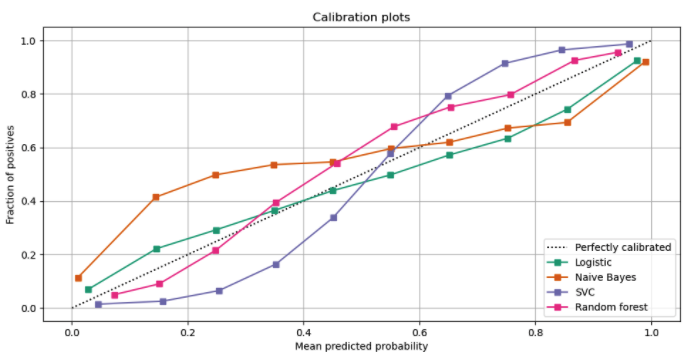
\includegraphics[width=0.55\textwidth]{figure_man/calibration.png}
\end{center}

\end{frame}

\begin{frame}{Calibration Plots}
\begin{itemize}
 %\item Logistic regression is already well-calibrated as it optimzes log-loss
 \item Many algorithms (except for logistic regression) return biased probabilities.
 \item Naive Bayes tends to push probabilities to 0 or 1 (see histograms in the graph).
 \item Random Forest classifier shows that probabilities close to the borders are very rare.
 %Base-level trees trained with random forests incorporate relatively high variance due to feature subsisting
 (Niculescu-Mizil and Caruana 2005).
 \item Linear SVC shows an even clearer sigmoid curve, because maximum-margin
 methods focus on the support vectors (close to the decision boundary).
\end{itemize}
\end{frame}



\begin{frame}{Calibration and Discrimination}
%<!-- http://www.uphs.upenn.edu/dgimhsr/documents/predictionrules.sp12.pdf -->
A well calibrated classifier can be poorly discriminating, e.g.

\begin{table}[]
\centering
\begin{tabular}{r|rrr}
\hline
Obs. Nr. & true $Y$ & $\fh_1$ & $\fh_2$ \\
\hline
1        & 1     & 1           & 0           \\
2        & 1     & 1           & 0           \\
3        & 0     & 0           & 1           \\
4        & 0     & 0           & 1           \\ \hline
Avg Prob & 50\%  & 50\%        & 50\%        \\
\hline
\end{tabular}
\end{table}

\begin{itemize}
  \item Both prediction rules ($\fh_1$ and $\fh_2$) result in the same calibration in the large (50\%).
  \item However, $\fh_1$ is better than $\fh_2$ as it correctly classifies the real outcome $Y$.
\end{itemize}

\end{frame}

\begin{frame}{Calibration and Discrimination}
A well discriminating classifier can have a bad calibration, e.g.

\begin{table}[]
\centering
\begin{tabular}{rrrr}
\hline
Obs. Nr. & truth $Y$ & $\fh_1$ & $\fh_2$ \\
\hline
1        & 1     & 0.9           & 0.9         \\
2        & 1     & 0.9           & 0.9           \\
3        & 0     & 0.1          & 0.7           \\
4        & 0     & 0.1         & 0.7           \\ \hline
Avg Prob & 50\%  & 50\%        & 80\%        \\
\hline
\end{tabular}
\end{table}

\begin{itemize}
  \item Both prediction rules are well discriminating, i.e., setting thresholds $c_1 = 0.5$ for $\fh_1$ and $c_2 = 0.8$ for $\fh_2$ perfectly separates positive and negative observations.
  \item Prediction rule 2 is rather poorly calibrated as the proportion of positive observations is estimated by $80\%$.
\end{itemize}

\end{frame}

\begin{frame}{Calibration and Discrimination}

{\centering 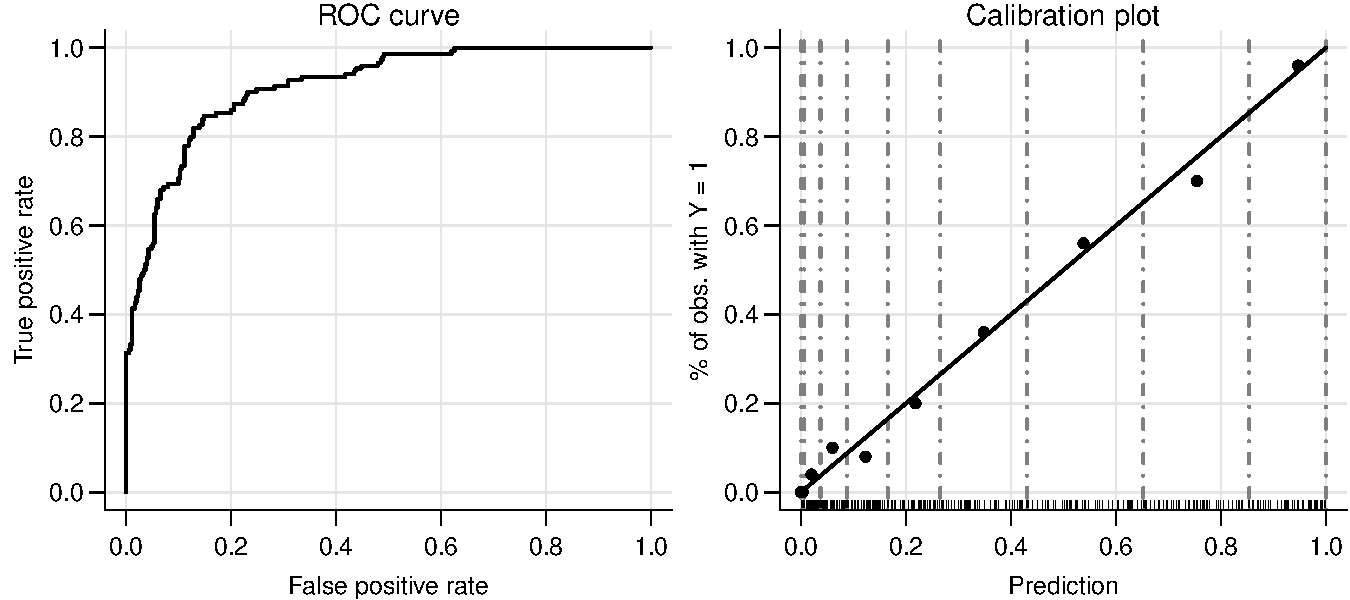
\includegraphics[width=\textwidth]{figure_man/calibdiscr1}}

% and do not visualize how well-calibrated the probabilities are.
%To assess the performance of classifiers, we should consider:
\begin{itemize}
\item \textbf{ROC curve:}
Measures only discrimination as it is based on TPR and FPR and assesses only the ranking of predicted probabilities (not their magnitude).
%Measures the ability to separate the classes well. % (e.g., confusion matrix). %accurately rank individuals from low to high risk.
\item \textbf{Calibration plot:} Measures (for reasonable groupings) how well the predicted probabilities match the proportion of positives. %(i.e., $Y = 1$).
\end{itemize}

\end{frame}

\begin{frame}{Calibration and Discrimination}

{\centering 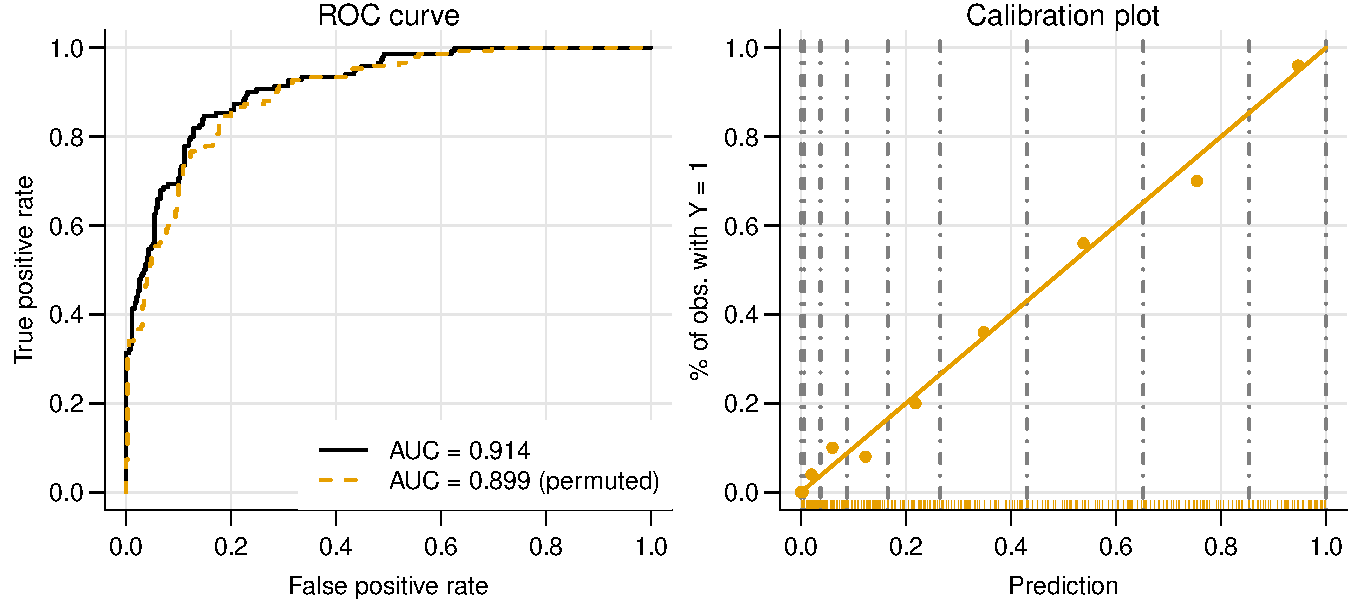
\includegraphics[width=\textwidth]{figure_man/calibdiscr2}}


\begin{itemize}
\item Permuting the predictions within each decile does not change the calibration plot.
\item However, the ROC curve and AUC can get worse as the ranking is changed.
\end{itemize}


\end{frame}

\begin{frame}{Calibration and Discrimination}

{\centering 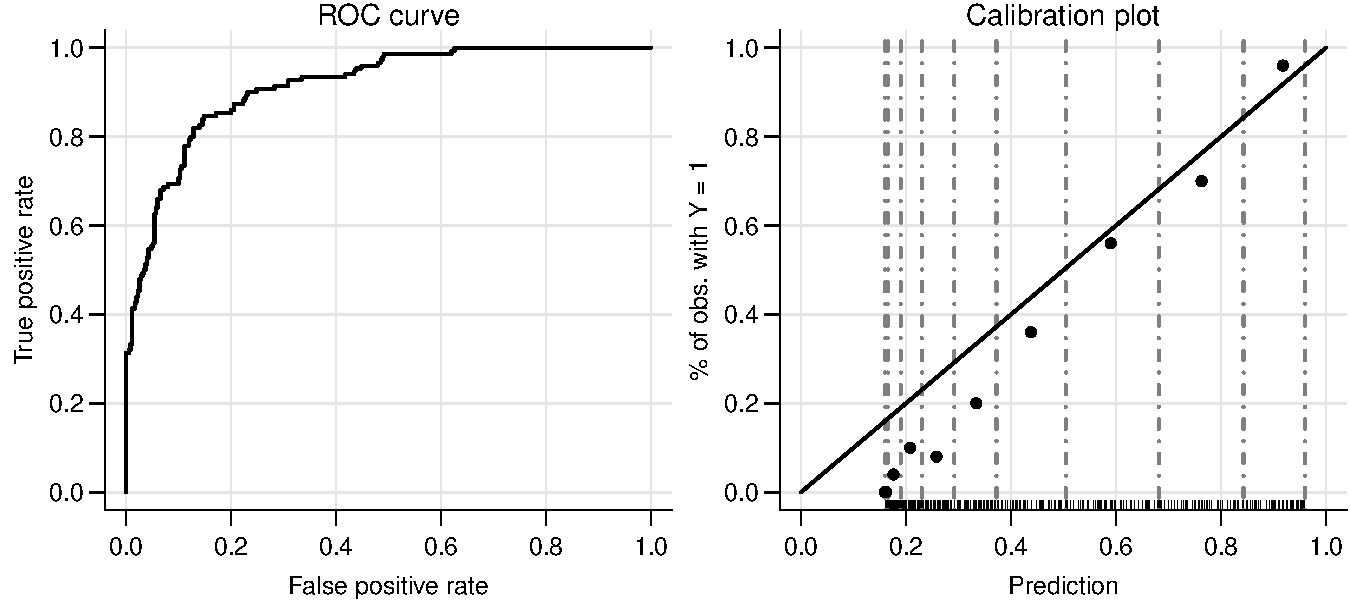
\includegraphics[width=\textwidth]{figure_man/calibdiscr3}}


\begin{itemize}
\item Monotonic transformations of the predicted probabilities do not change the ROC curve as the ranking will not change.
\item However, the calibration plot looks worse as the probabilities are shifted.
\end{itemize}
\end{frame}



\begin{frame}{Calibrating Probabilities}

\begin{itemize}
  \item Calibrating probabilities means to post-process the predictions to improve the estimates and obtain more reliable probabilities.
  %\item Two popular calibration methods are the \textbf{Platt’s scaling} (parametric) and the \textbf{isotonic regression} (non-parametric).
  \item A well calibrated classifier should classify samples such that among these samples with a predicted probability of 0.7, approximately 70\% actually belong to the positive class.
  \item The link function of logistic regression is basically a calibration for the scores predicted by linear regression.
  \item Note that calibration should be performed on new data not used for model fitting.
\end{itemize}

%In order to extract exact probabilities, like logarithmic loss does, a classifier can be calibrated, i.\,e. the output score of the calssifier can be transformed into a more accurate probability. The link function of logisitc regression is basically a calibration for the linear regression. In order to evaluate the calibration an additional validation data set is used. \lz
\end{frame}

\begin{frame}{Calibrating Probabilities}

The \textbf{Platt's scaling} (parametric sigmoid calibration) and the \textbf{isotonic regression} (non-parametric) are popular calibration methods:
\begin{itemize}
\item \textbf{Platt's scaling:} logistic regression on the output of the classifier with respect to the true class labels.
\item \textbf{Isotonic regression:} fit a piecewise-constant non-decreasing function instead of logistic regression.
\end{itemize}

%\tiny{Source 1: https://scikit-learn.org/stable/modules/calibration.html}
%\tiny{Source 2: http://fastml.com/classifier-calibration-with-platts-scaling-and-isotonic-regression/}
%\tiny{Source 3: https://towardsdatascience.com/probability-calibration-for-boosted-trees-24cbd0f0ccae}
%\tiny{Source 3: https://jmetzen.github.io/2015-04-14/calibration.html}
%\tiny{Source 4: http://fa.bianp.net/blog/2013/isotonic-regression/}
%\tiny{Source 5: https://www.analyticsvidhya.com/blog/2016/07/platt-scaling-isotonic-regression-minimize-logloss-error/}


\textbf{Platt's scaling}:

\begin{itemize}
  \item Train a logistic regression model using the (uncalibrated) classifier's predictions $\hat{Y}$ as input and the true labels as output.
  \item Use the probabilities $\hat{\pi}$ of this logistic regression model as calibrated predictions.
  %\item Essentially Platt's scaling performs a logistic regression on the output of a classifier.
\end{itemize}
% \begin{center}
% \includegraphics[width=0.55\textwidth]{figure_man/platt.png}
% \end{center}


\end{frame}


\begin{frame}{Platt's Scaling}

\begin{figure}
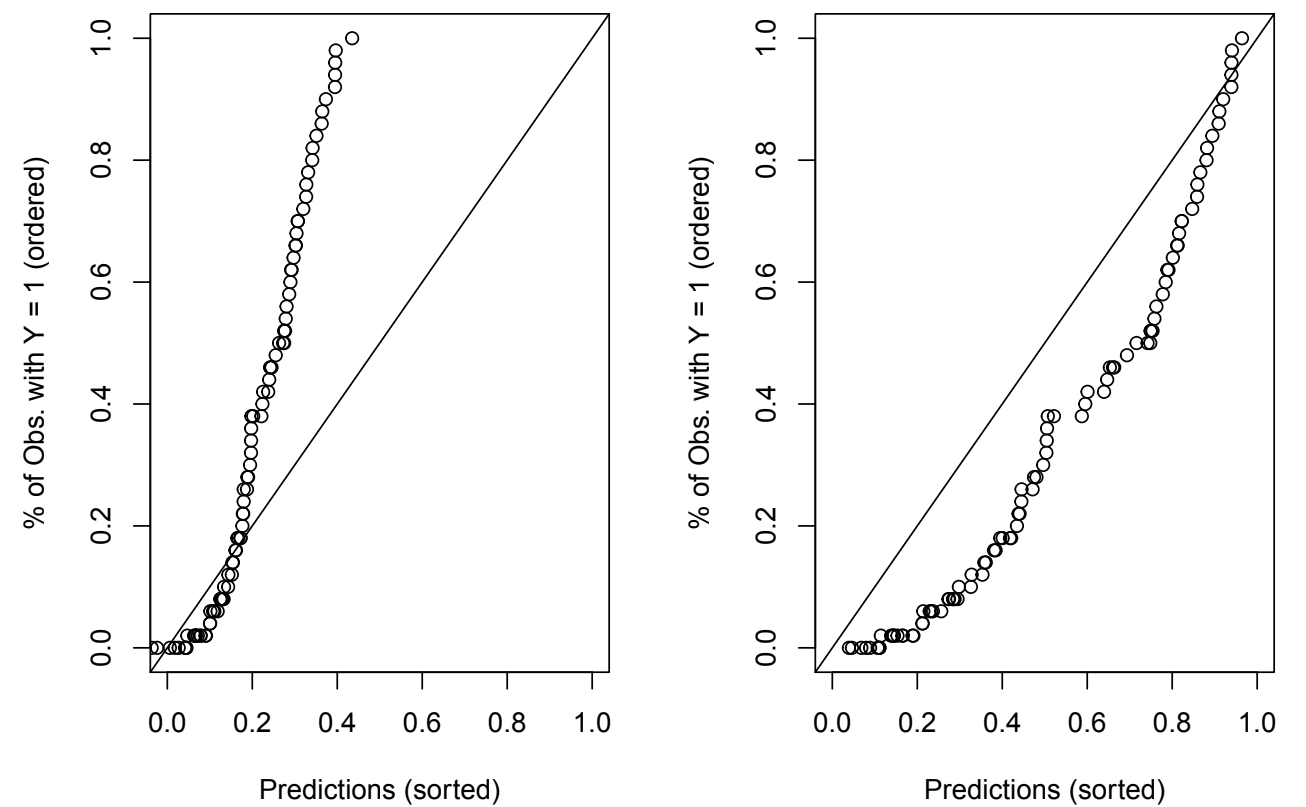
\includegraphics[width=0.8\textwidth]{figure_man/platts-scaling.png}
\end{figure}

\end{frame}


\begin{frame}{Isotonic regression}

\begin{itemize}
\item The idea is to fit a piecewise-constant non-decreasing function instead of
logistic regression with the pool adjacent violators algorithm
($\mathcal{O}(n)$).
\item Basically, the algorithm goes through the data and looks for violations of
the monotonicity constraint. If it finds one, it gets adjusted with the best
possible fit under the constraint.
\end{itemize}

\begin{center}
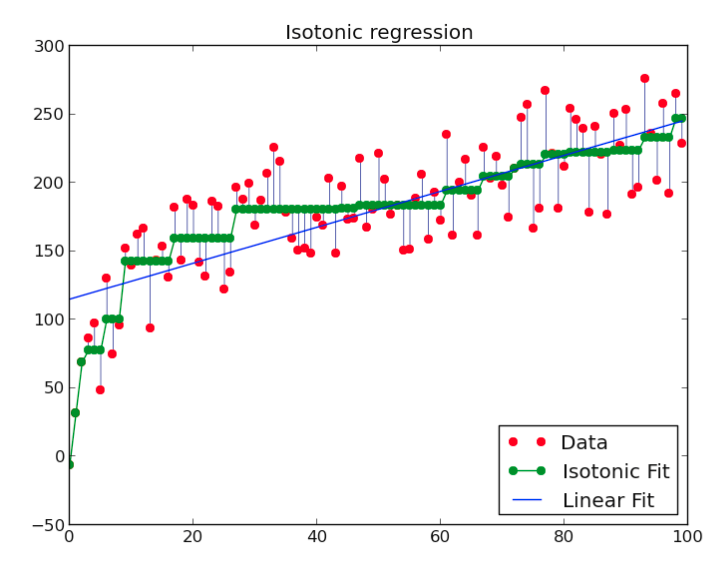
\includegraphics[width=0.5\textwidth]{figure_man/iso-reg.png}
\end{center}
\end{frame}
\begin{frame}{Isotonic regression}

\begin{figure}
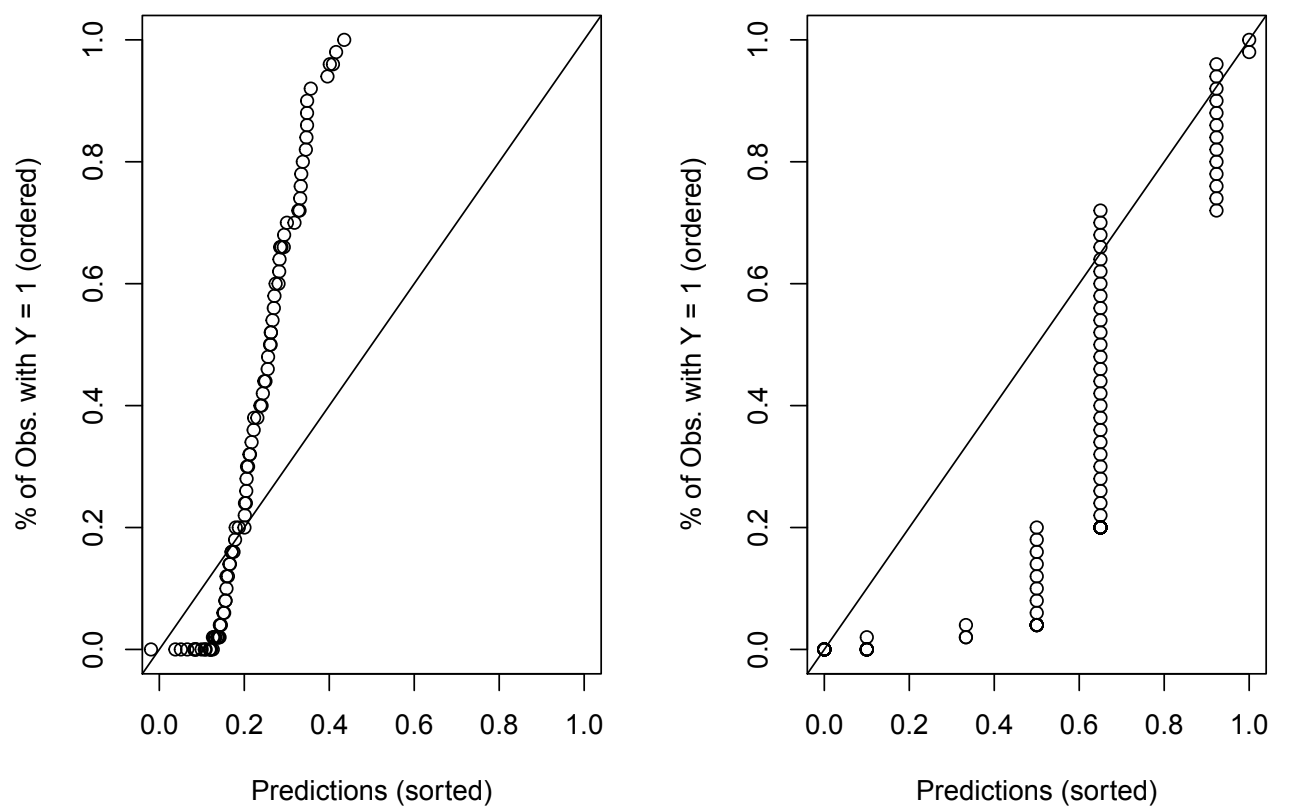
\includegraphics[width=0.8\textwidth]{figure_man/isotonic-reg.png}
\end{figure}

\end{frame}


\begin{frame}{Example: Calibration Plot}

Calibrating a SVC with Platt's scaling and isotonic regression:
\begin{center}
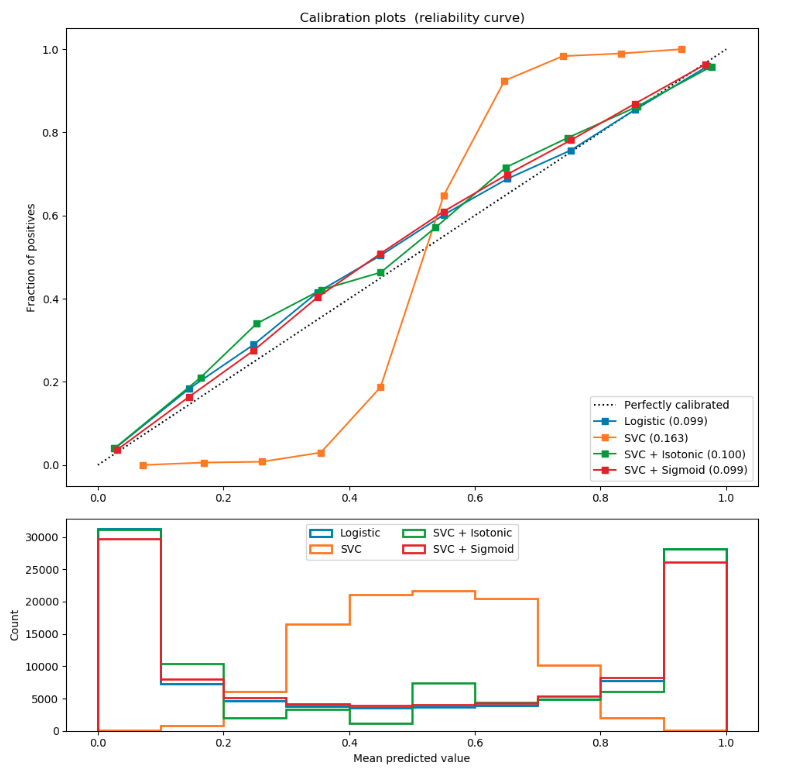
\includegraphics[width=0.6\textwidth]{figure_man/calibration2.png}
\end{center}

\end{frame}
% 
% \section{Sharpness}
% 
% 
% \begin{frame}{Sharpness}
% 
% \begin{itemize}
% \item Sharpness is the concentration of the predictive distributions, an exclusive measure of the forecasts 
% \item For density forecasts for a real-valued variable, sharpness can be assessed in terms of the associated prediction intervals. The mean widths of these intervals should be as short as possible, subject to the empiricalcoverage being at the nominal level.
% \end{itemize}
% 
% \end{frame}


\section{Proper Scoring Rules}

\begin{frame}{Proper Scoring Rules}

\begin{itemize}
\item Proper scoring rules are specific loss functions to evaluate probabilistic forecasts
\item These allow to \textbf{quantify} the goodness of calibration by a numerical score 
\begin{itemize}
\item positively-orientied (p.o.) scoring rules:  higher values $=$ better 
\item negatively-oriented (n.o.) scoring rules: lower values $=$ better 
\end{itemize}
%\item We start with the definition for a continuous outcome $Y \in \Yspace$ % = \{1, ..., g\}$
\item A \textbf{scoring rule} assigns a score $S(Q, y) \in \mathbb{R} \cup \{-\infty, \infty \}$ to each pair of 
\begin{itemize}
\item predictive probability distribution $Q \in \mathcal{F}$ from a class of CDFs
\item and realized valued $y$ of $Y \sim \mathbb{P}_y$.
\end{itemize}
\item $S$ may also depend on the density / PDF $q$ corresponding to $Q$

% $$
%   Q = \left(\pi_1, ..., \pi_g\right), \quad \sum_i \pi_i = 1
% $$


\item Accessing properties of scoring rules is therefore only possible after observing $Y=y$

\item We therefore look at the expected value of scoring rule
\end{itemize}
\end{frame}
\begin{frame}{Proper Scoring Rules}
\begin{itemize}
\item We say a n.o. scoring rule $S$ is \textbf{proper} relative to $\mathcal{F}$ if the expected {score}

$$
\mathcal{S}(\mathbb{P}_y, Q) := \E_{y \sim \mathbb{P}_y}[S(Q, Y)]
$$

is maximized for $Q = \mathbb{P}_y$, i. e. 

$$
\mathcal{S}(\mathbb{P}_y, \mathbb{P}_y) \le \mathcal{S}(\mathbb{P}_y, Q). 
$$
\item That means, that if we believe that $\mathbb{P}_y$ is the best forecast we are also incentivized to report $\mathbb{P}_y$ (and no other $Q$ in order to achieve a better score). 
\item In practice, algorithms are then compared using averaged scores for all observations
\end{itemize}

% 
% 
%  The expected score is then
% 
% $$
%   S(P, Q)
% $$
% 
% \lz
% 
% In general, one aims at finding a scoring rule that gives the \textbf{highest expected reward} if the probabilistic forecast $Q$ corresponds to the true underlying probability $P$ (\enquote{encourage} the forecaster to be \enquote{honest}).
% 
% 
% If the highest \textbf{} \textbf{proper scoring rule}
% 
% 
% 
% A \textbf{Scoring Rule} $S$ is a function to assess the performance of a probability forecast.
% \medskip
% 
% \textbf{Formal definition:}\\
% Let $P \in \mathcal{P}$ be a probability forecast, $y \in \Yspace$ the observed outcome then
% $$
% S: \mathcal{P} \times \Yspace \to \R \cup \{-\infty, \infty\}, \quad S(P, y)
% $$
% is called Scoring Rule.
% \medskip
% 
% Since $S(P, y)$ depends on the single observed outcome $y$, we can specify the expected score assuming the true distribution $Q$ as
% $$
% S(P,Q) = \int S(P,y) dQ(y)
% $$
% \framebreak
% 
% \textbf{Proper Scoring Rule:}\\
% A Proper Scoring Rule should incentivize the forecaster to strictly report the outcome of his model.
% \medskip
% 
% \textbf{Formal definition:}\\
% Assume $Q \in \mathcal{P}$, for the Proper Scoring Rule the following holds
% $$
% S(P, P) \leq S(P,Q) ,\forall P, Q \in \mathcal{P}
% $$
% \framebreak

\end{frame}


% \begin{frame}{Proper Scoring Rule for Discrete Outcomes}
% 
% For \textit{discrete outcomes} we can define proper scoring rules via the \textit{Savage representation}.
% \medskip
% 
% Therefore we assume the sample space $\Yspace = \{1,...,g\}$ with g mutually exclusive events. The respective probability forecast for this space is represented by $p = (p_{1},...,p_{g})^{T}$ where $p_{i}$ is the probability that event $i$ occurs. The set of probability measures can be stated as
% \begin{align*}
% \mathcal{P} = \{p = (p_{1},...,p_{g})^{T}: p_{1},...,p_{g} \geq 0, p_{1}+...+p_{g} = 1  \}
% \end{align*}
% 
% \end{frame}

\begin{frame}{Commonly used Proper Scoring Rules}

Let $q$ be the corresponding density / PDF of $Q$\\

\vspace*{0.4cm}
\textbf{For continuous outcome}:
\begin{itemize}
\item Negative Logarithmic Score: 
$$S_{LS}(q,y) = -\log(q(y))$$
\item Brier / Quadratic Score:
$$S_{QS}(q,y) = -2q(y) + \int q^2(y) dy$$
\end{itemize}

\end{frame}

\begin{frame}{Commonly used Proper Scoring Rules}

\textbf{For discrete outcome}:
\begin{itemize}
\item Brier Score for binary outcome: 
$$S_{BS}(q,y) = (y-q(y))^2$$
\item Continuous Ranked Probability Score: 
$$S_{CRPS}(Q,y) = \int (Q(x) - I(x \leq y))^2 dx$$
with $I(\cdot)$ the the indicator function
\end{itemize}

\end{frame}


\begin{frame}{Example}

\textbf{Brier and Log Score vs. improper Scoring Rules}

\begin{itemize}
\item $Y \sim \mathcal{B}er(\pi \sim \mathcal{B}eta(0.1,0.1))$
\item Models for probabilistic forecast:
\begin{itemize}
\item Model 1: Oracle discriminator $$\hat{\pi} = 0.01 \cdot (y-0.5) + 0.5,$$ but not well calibrated
\item Model 2: Oracle for probabilites $\hat{\pi} = \pi$
\item Model 3: Use $\mathbb{P}_y$
\end{itemize}
\end{itemize}


\small
\begin{center}
\begin{tabular}{cccc}
\hline
    & 1-AUC & BS & LS\\
\hline
Model 1 & 0.00 & 0.25 & 0.68\\
Model 2 & 0.02 & 0.05 & 0.17\\
Model 3 & 0.00 & 0.00 & -0.00\\
\hline
\end{tabular}
\end{center}

\small
\vspace{0.2cm}
Exercise: Proof, that AUC is not a proper scoring rule.

\end{frame}


% \begin{frame}{Are they all the same?}

% http://arogozhnikov.github.io/2016/07/12/secret-of-ml.html

% \end{frame}


\endlecture
\end{document}
